\newif\ifglobal

%%%%%%%%%%%%%%%%%%%%%%%
%%% Compile to view %%%
%%%%%%%%%%%%%%%%%%%%%%%

%%%%%%%%%%%%%%%%%%%%%%%%%%%%%%%%%%%%%%%%%%%%%%%%%%%
%%% Readme:                                     %%%
%%% https://www.overleaf.com/read/bwdjvfjksvjy/ %%%
%%%%%%%%%%%%%%%%%%%%%%%%%%%%%%%%%%%%%%%%%%%%%%%%%%%

% >>> M?: marks a module setting number or important notice

% >>> M4: Set {./relative-path} to external files for this module <<<
\def \modulefiles {./38-WCTRL}
% To add an external file, use:
% (Replace '---' with actual filename)
% '\input{\modulefiles/tables/---.tex}' for tables
% '\includegraphics{\modulefiles/figures/---}' for figures
% '\subfile{\modulefiles/---}' for register files

% >>> M1: This module is in global project? <<<
% 'YES' - uncomment; 'NO' - comment out
\globaltrue

\ifglobal
    \documentclass[main\_\_CN.tex]{subfiles}

\else
    % Font "FandolSong-Regular" used by ctex does not have GSUB table.
    % It causes warnings that do not affect compilation and can be ignored.
    \PassOptionsToPackage{quiet}{fontspec}

    \documentclass[openany, 10pt]{book}

    % >>> M2: In ./00-shared/preamble-trm-module, also find
    %         settings for visibility of todo notes, watermark <<<
    \usepackage{preamble-trm-module}


    % Enable Chinese typesetting
    \usepackage{ctex}

    % >>> M3: Temporary labels in Chinese
    %         you can add your own labels there <<<
    \myexternaldocument{./00-shared/temp-labels-cn}

\fi %\ifglobal


\setcounter{secnumdepth}{4}

% >>> M5: If this module needs any updates in
% './00-shared/preamble-trm-module.sty'
% (include additional package, etc.), contact your module PM
% or create the file './00-shared/changelog.tex' make the
% necessary updates yourself and document them in this file <<<


\begin{document}


% Sets language into which pre-defined bits of text are translated
\selectlanguage{chinese}

% Do not delete this block
\ifglobal
% Add the following front matter if
% this module is outside of global project
\else
    \InputIfFileExists{readme}{}{}
    {\let\clearpage\relax \listoftodos}
    \tableofcontents
    %\listoftables
    %\listoffigures
\fi


%%%%%%%%%%%%%%%%%%%%%%%%%
%%% TRM Module Begins %%%
%%%%%%%%%%%%%%%%%%%%%%%%%

\hypertarget{wctrl}{}
\chapter{World 控制器 (WCL)}\label{mod:wctrl}

\section{概述}

\chipname{} 允许用户将芯片的硬件和软件资源分为安全世界 (World0) 和非安全世界 (World1)，从而有效防止非法数据拷贝、破坏或篡改，或通过恶意软件、硬件监视、硬件干预等方式破坏或获取设备信息。两个世界之间可以由 World 控制器进行切换。

默认情况，\chipname{} 不划分安全世界和非安全世界，所有资源全部共享。如有需求，用户可通过权限配置将资源分为安全世界和非安全世界，具体配置请见章节 \ref{mod:permctrl} \textit{\nameref{mod:permctrl}}，本章节仅介绍 World 控制器及 CPU 在两个世界之间的切换。

\section{主要特性}
\label{sec:alias-features}

\chipname{} 的 World 控制器主要用于：
\begin{itemize}
    \item 控制 CPU 在安全世界与非安全世界中的相互切换
    \item 记录 CPU 的世界切换信息
    \item 屏蔽 CPU 的 NMI 中断
    \item 两个 CPU（CORE\_\regindex{m}：CPU0 和 CPU1）可独立切换
\end{itemize}

\section{功能描述}
\label{sec:38-WCTRL-func-descr}

在 World 控制器的帮助下，\chipname{} 的安全世界和非安全世界可以访问的资源可以不同：

\begin{itemize}
    \item 安全世界 (World0)：
    \begin{itemize}
        \item 可以访问所有的外设和存储空间。
        \item 主要执行所有需要保密的操作，如指纹识别、密码处理、数据加解密、安全认证等。
    \end{itemize}
    \item 非安全世界 (World1)：
    \begin{itemize}
        \item 只能访问部分的外设和存储空间。
        \item 执行其他操作，如用户操作系统、各种应用程序等。
    \end{itemize}
\end{itemize}


\chipname{} 的 CPU 和从设备均有相应的安全世界和非安全世界权限：
\begin{itemize}
    \item CPU 可以在两个世界中运行：
        \begin{itemize}
            \item 在安全世界：运行安全世界的程序
            \item 在非安全世界：运行非安全世界的程序
            \item CPU 上电时均默认处于安全世界，此后可配置通过 World 控制器在两个世界间进行切换。
        \end{itemize}
    \item 所有的从设备（外设\hyperref[note:wctrl-access]{*}、存储器等）均可分别配置：
        \begin{itemize}
            \item 安全世界权限：表示可以从安全世界访问，即允许 CPU 从安全世界中访问该从设备；
            \item 非安全世界权限：表示可以从非安全世界访问，即允许 CPU 从非安全世界中访问该从设备。
            \item 注意，从设备可配置为同时具有安全世界和非安全世界权限。
        \end{itemize}
        具体请见章节 \ref{mod:permctrl} \textit{\nameref{mod:permctrl}}。
\end{itemize}

\begin{tiplisting}\label{note:wctrl-access}
World 控制器本身也属于一种外设。因此，与所有从设备一样，World 控制器理论上也可以配备安全世界和非安全世界的访问权限，即允许从安全世界和非安全世界访问 World 控制器。不过，为了保证世界切换的安全性，应\textbf{禁止} World 控制器的非安全世界访问权限，确保 CPU 无法从非安全世界中更改 World 控制器的配置。
\end{tiplisting}

\textbf{CPU 在访问从设备时：}

\begin{enumerate}
    \item 首先，CPU 将告知从设备自己所处的世界；
    \item 接着，从设备会根据自身的权限配置，判断是否允许 CPU 的访问。
        \begin{itemize}
        \item 如果允许访问，则访问继续；
        \item 如果不允许访问，则不响应此次访问并且触发中断。
        \end{itemize}
\end{enumerate}
这样一来，可以保证安全世界的资源不会被非安全世界非法访问。

\section{CPU 的世界切换} \label{sec:38-WCTRL-recommended-operation}

CPU 可以从安全世界切换至非安全世界，也可以从非安全世界切换至安全世界。

\subsection{安全世界切换到非安全世界}\label{sec:38-WCTRL-safe-nosafe-switch}

\begin{figure}[H]
    \centering
    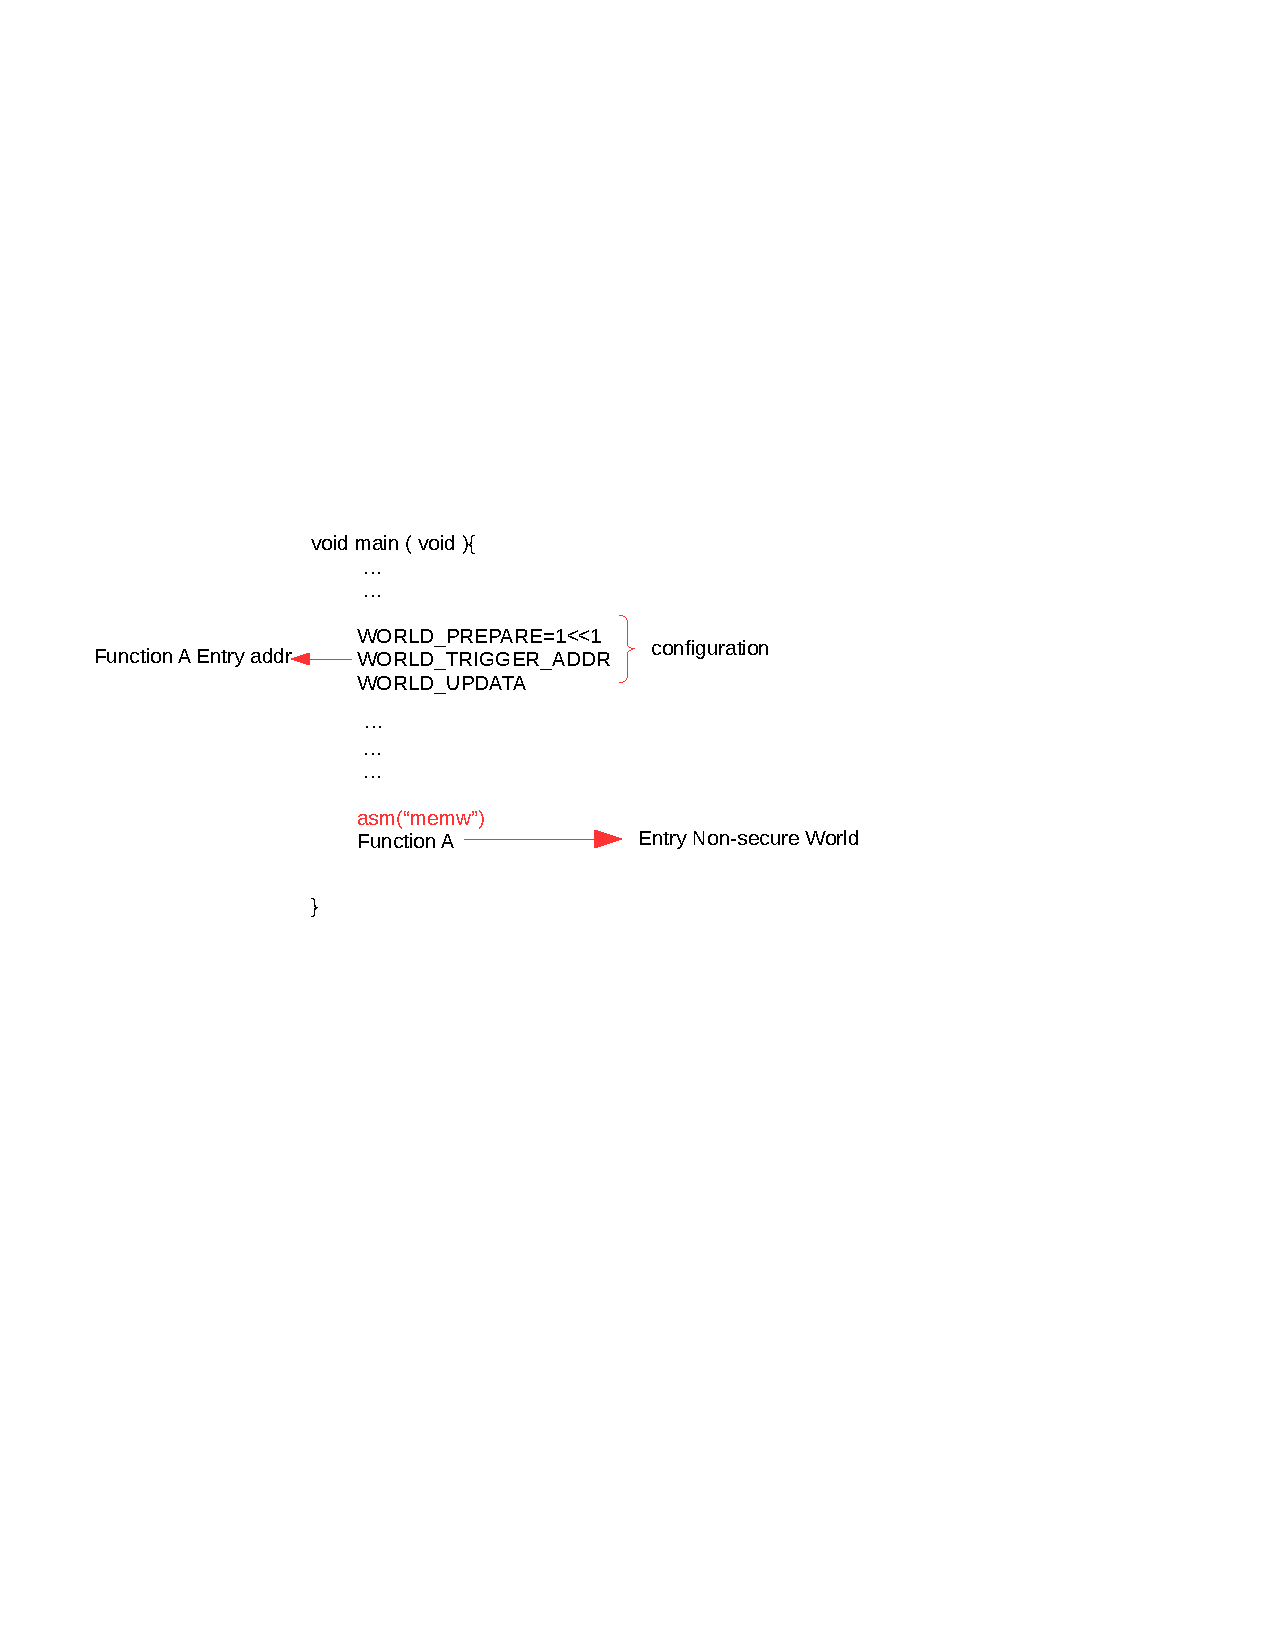
\includegraphics[width=0.7\textwidth]{./38-WCTRL/figures/world0toworld1.pdf}
    \caption{安全世界切换到非安全世界}
    \label{fig:38-WCTRL-safe-nosafe-switch}
\end{figure}

当\chipname{} 的 CPU 准备从安全世界执行非安全世界程序时，只需完成如下步骤：
\begin{enumerate}
    \item 配置 World 控制器，详见下方描述。
    \item 冲刷 write\_buffer 中残留的数据，详见第 \ref{sec:wctrl-writer-buffer} 小节。
\end{enumerate}

完成以上操作后，即可调用非安全世界的程序。

但值得注意的是，由于存在预取指和流水线等方面原因，如果在 World 控制器配置完成后立即调用非安全世界程序，则可能存在配置程序尚未运行完成，但 CPU 已经执行了非安全世界应用程序的情况。这样一来，World 控制器将一直无法检测到 CPU 读取入口地址的行为，从而无法切换至非安全世界，导致非安全世界的程序在安全世界中运行，带来安全风险。

因此，一定要确保配置程序运行完成后，再调用非安全世界应用程序。具体来说，可以\textbf{将非安全世界应用程序申明为 noinline 属性}。


\subparagraph{配置 World 控制器}

World 控制器的具体配置过程如下：
\begin{enumerate}
    \item 配置 \hyperref[regdesc:WCLCORE0WORLDPREPAREREG]{WCL\_CORE\_\regindex{m}\_WORLD\_PERPARE\_REG} 寄存器为 0x{}2，表示要切换至进入非安全世界。
    \item 配置 \hyperref[regdesc:WCLCORE0WORLDTRIGGERADDRREG]{WCL\_CORE\_\regindex{m}\_World\_TRIGGER\_ADDR\_REG} 寄存器为非安全世界的入口地址，即需要执行的非安全世界应用程序的入口地址。
    \item 配置 \hyperref[regdesc:WCLCORE0WORLDUPDATEREG]{WCL\_CORE\_\regindex{m}\_World\_UPDATE\_REG} 寄存器（可配置任意值），代表已完成配置。
\end{enumerate}

\begin{tiplisting}\label{note:38-WCTRL-safe2unsafe}
\vspace{-2em}
\begin{itemize}
    \item 注意 \hyperref[regdesc:WCLCORE0WORLDPREPAREREG]{WCL\_CORE\regindex{m}\_WORLD\_PERPARE\_REG} 和 \hyperref[regdesc:WCLCORE0WORLDTRIGGERADDRREG]{WCL\_CORE\_\regindex{m}\_World\_TRIGGER\_ADDR\_REG} 的配置前后顺序不作要求，\hyperref[regdesc:WCLCORE0WORLDUPDATEREG]{WCL\_CORE\_\regindex{m}\_World\_UPDATE\_REG} 寄存器必须最后配置。
    \item 配置完成后，需要使用 memw (memory wait) 汇编指令清除 write\_buffer，详情请见第 \ref{sec:wctrl-writer-buffer}。
\end{itemize}
\end{tiplisting}

此后，World 控制器会持续检测 CPU 是否执行到配置的应用程序入口：一旦检测到 CPU 开始从配置的入口地址取指，则会将 CPU 切换至非安全世界，并开始从非安全世界中执行应用程序。

需要注意的是，World 控制器经过配置后：
\begin{itemize}
    \item 将持续进行检测，直至检测到 CPU 开始从配置的入口地址取指，则从安全世界切换至非安全世界。
    \begin{itemize}
        \item 如需取消配置，可通过配置 \hyperref[regdesc:WCLCORE0WORLDCANCELREG]{WCL\_CORE\_\regindex{m}\_World\_Cancel\_REG} 寄存器取消，此时即使 CPU 执行到了配置的入口地址处，也不会触发世界切换。注意配置完成后，同样需要使用 memw (memory wait) 汇编指令清除 write\_buffer，详情请见第 \ref{sec:wctrl-writer-buffer}。
    \end{itemize}
    \item 每次生效后将自动停止检测。因此，每次从安全世界切换到非安全世界都需要重新配置。
\end{itemize}


\subsection{非安全世界切换到安全世界}\label{sec:38-WCTRL-nosafe-safe-switch}

\begin{figure}[H]
    \centering
    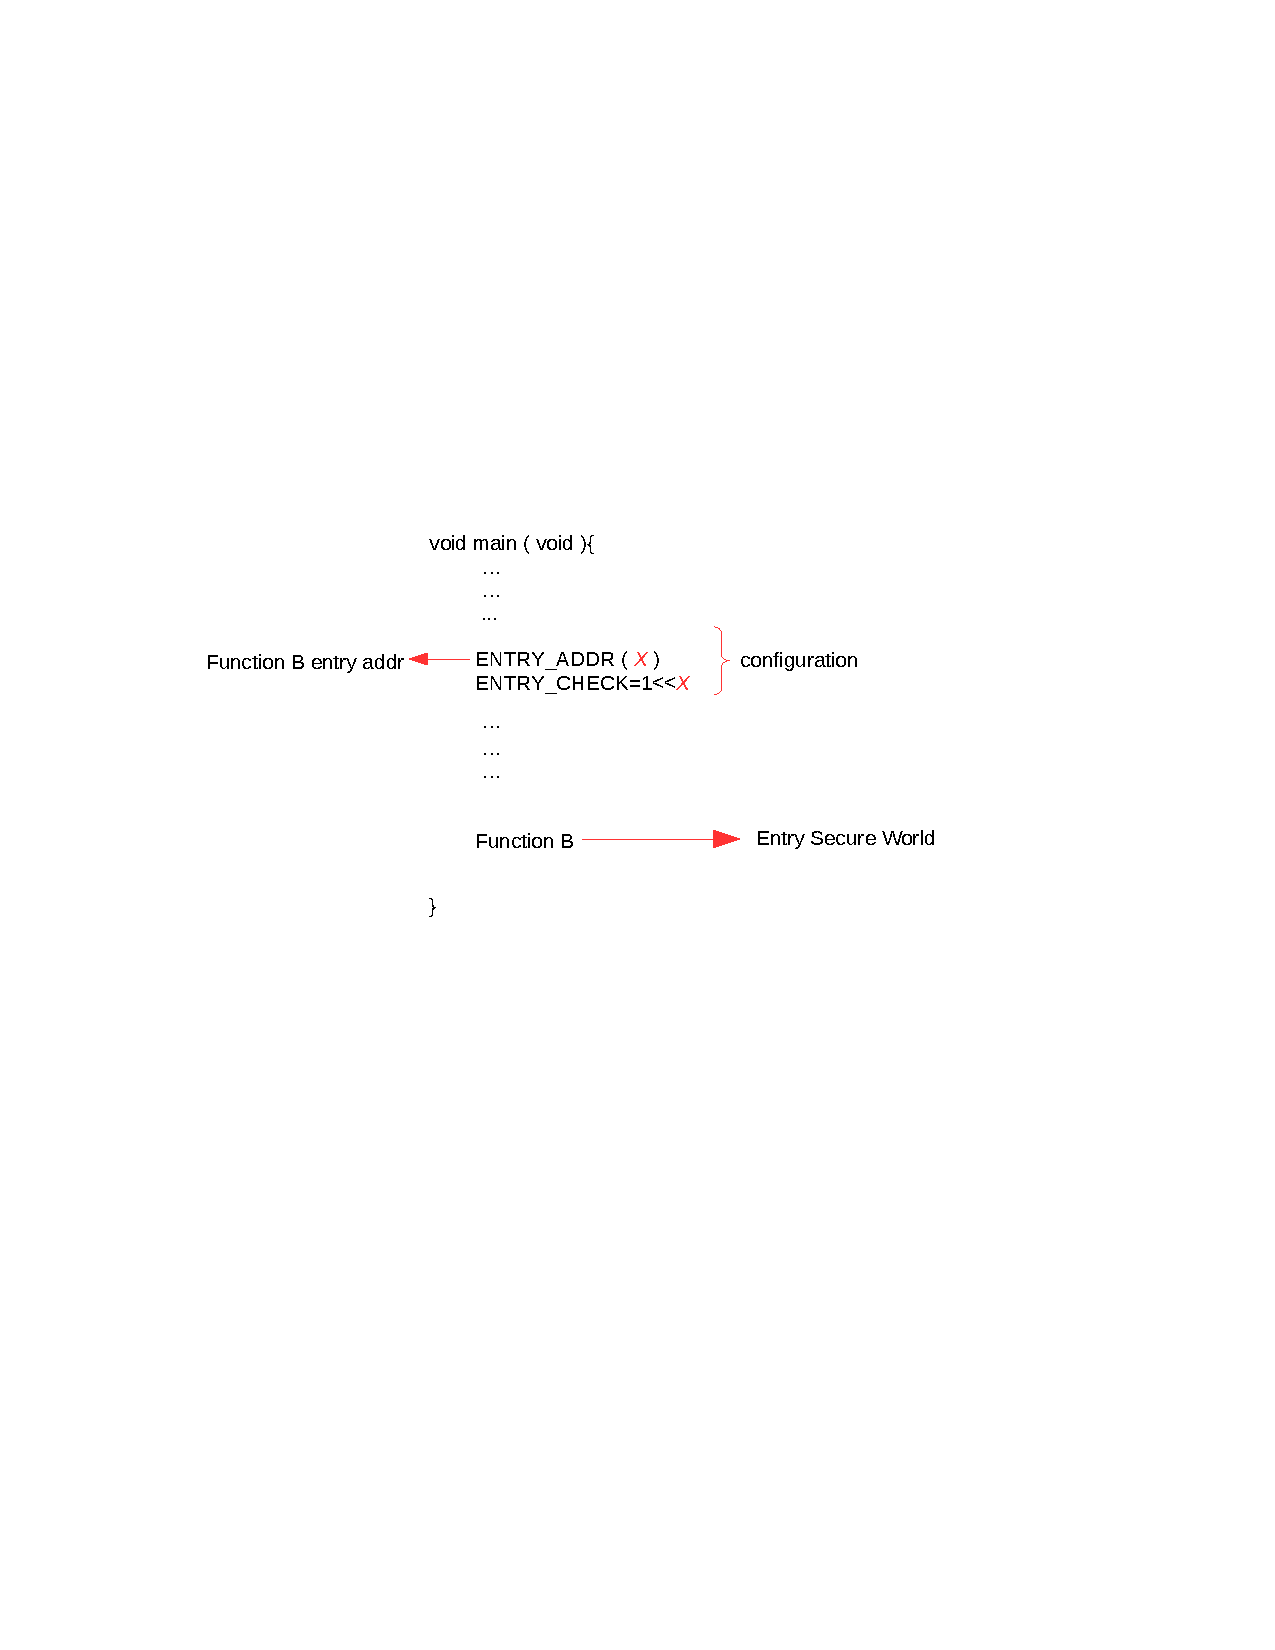
\includegraphics[width=0.7\textwidth]{./38-WCTRL/figures/world1toworld0.pdf}
    \caption{非安全世界切换到安全世界}
    \label{fig:38-WCTRL-nosafe-safe-switch}
\end{figure}

当 CPU 结束非安全世界应用程序，准备切换执行安全世界程序时：需要通过触发\textbf{中断}和\textbf{异常}的方式。经过配置后，当 World 控制器检测到触发的中断或异常后，会自动切换到安全世界中。

具体流程如下：

\begin{enumerate}
    \item 配置 \hyperref[regdesc:WCLCORE0MESSAGEADDRREG]{WCL\_CORE\_\regindex{m}\_MESSAGE\_ADDR\_REG} 和 \hyperref[regdesc:WCLCORE0MESSAGEMAXREG]{WCL\_CORE\_\regindex{m}\_MESSAGE\_MAX\_REG} 寄存器清除 write\_buffer，详见 \ref{sec:wctrl-writer-buffer}。
    \item 配置 \hyperref[regdesc:WCLCORE0ENTRYnADDRREG]{WCL\_CORE\_\regindex{m}\_ENTRY\_\regindex{n}\_ADDR\_REG (\regindex{n}: 1-13)} 为各级中断或异常的入口地址。
    \begin{itemize}
        \item 由于 \chipname{} 所有的中断和异常的入口地址都是基于 VecBase 特殊寄存器（基地址）+ 固定偏移，因此每次修改 VecBase 特殊寄存器时都需要重新配置入口地址。
    \end{itemize}
    \item 配置 \hyperref[regdesc:WCLCORE0ENTRYCHECKREG]{WCL\_CORE\_\regindex{m}\_ENTRY\_CHECK\_REG} 使能对任意入口地址的监测，一旦 CPU 执行到监控的入口地址处即立刻将 CPU 切换到安全世界。
    \begin{itemize}
        \item 第 \regindex{x} 比特控制对 \regindex{x} 号入口 \hyperref[regdesc:WCLCORE0ENTRYnADDRREG]{WCL\_CORE\_\regindex{m}\_ENTRY\_\regindex{x}\_ADDR\_REG} 的监测，可配置为同时监测多个入口
        \begin{itemize}
            \item 0: 禁用监测
            \item 1: 开始监测
        \end{itemize}
        \item \hyperref[regdesc:WCLCORE0ENTRYCHECKREG]{WCL\_CORE\_\regindex{m}\_ENTRY\_CHECK\_REG} 寄存器一次使能，长期有效。之后每次监测到入口地址的取指行为都会自动切换到安全世界，直至被禁用。
    \end{itemize}
\end{enumerate}

\subsection{清除 write\_buffer}\label{sec:wctrl-writer-buffer}

由于 \chipname{} 的 \href{https://en.wikipedia.org/wiki/Write_buffer}{write\_buffer} 机制，因此在 CPU 切换世界时，总线上可能还残留另一个世界的信息并执行另一个世界的操作。为保证安全，必须在世界切换时，对 writer\_buffer 进行冲刷，具体方法有两种：
\begin{itemize}
    \item \textbf{安全世界切换至非安全世界时}：
    \begin{itemize}
        \item 使用 memw 汇编命令。
    \end{itemize}
    \item \textbf{从非安全世界进入安全世界时}：
    \begin{itemize}
        \item 切换 CPU 数据总线：
            \begin{enumerate}
        \item 预配置以下寄存器：
        \begin{itemize}
            \item \hyperref[regdesc:WCLCORE0MESSAGEADDRREG]{WCL\_CORE\_\regindex{m}\_MESSAGE\_ADDR\_REG} 为一段非安全世界的地址；
        \item \hyperref[regdesc:WCLCORE0MESSAGEMAXREG]{WCL\_CORE\_\regindex{m}\_MESSAGE\_MAX\_REG} 为 \regindex{Z} (\begin{math} Z \in \{ 3, 4, \dots, 16 \end{math}\})
        \end{itemize}
        \item 每次切换世界时均向 \hyperref[regdesc:WCLCORE0MESSAGEADDRREG]{WCL\_CORE\_\regindex{m}\_MESSAGE\_ADDR\_REG} 配置的地址中连续写入 0、1、\dots 、\regindex{Z-1}、\regindex{Z} 这个序列。比如，\regindex{Z} 若配置为 3，则连续写入 0、1、2、3 这四个数字；如 \regindex{Z} 配置为 5，则连续写入 0、1、2、3、4、5。
        \item 此后，当硬件检测到 \hyperref[regdesc:WCLCORE0MESSAGEADDRREG]{WCL\_CORE\_\regindex{m}\_MESSAGE\_ADDR\_REG} 配置的地址中开始连续写入 \\ \hyperref[regdesc:WCLCORE0MESSAGEMAXREG]{WCL\_CORE\_\regindex{m}\_MESSAGE\_MAX\_REG} 中约定的序列时，则将立即切换 CPU 数据总线至另一个世界。
    \end{enumerate}
    \end{itemize}
\end{itemize}



















\section{世界切换记录表} \label{subsub:world_switch_table}

通常情况下，CPU 会频繁进行世界切换且存在中断嵌套。为了能够回溯到切换至安全世界之前的世界属性，World 控制器还会自动记录世界切换日志，并将其保存在一系列寄存器中，即“世界切换记录表”。


\subsection{世界切换记录表寄存器的组成}

世界切换记录表由 13 个 \hyperref[regdesc:WCLCORE0STATUSTABLEnREG]{WCL\_CORE\_\regindex{m}\_STATUSTABLE\regindex{n}\_REG(\regindex{n}: 1-13)} 寄存器组成（结构如图 \ref{fig:wcl-world-status} 所示），其中 \hyperref[regdesc:WCLCORE0STATUSTABLEnREG]{WCL\_CORE\_\regindex{m}\_STATUSTABLE\regindex{x}\_REG} 寄存器记录 \regindex{x} 号入口 \hyperref[regdesc:WCLCORE0ENTRYnADDRREG]{WCL\_CORE\_\regindex{m}\_ENTRY\_\regindex{x}\_ADDR\_REG} 的世界切换情况。

\begin{figure}[H]
    \centering
    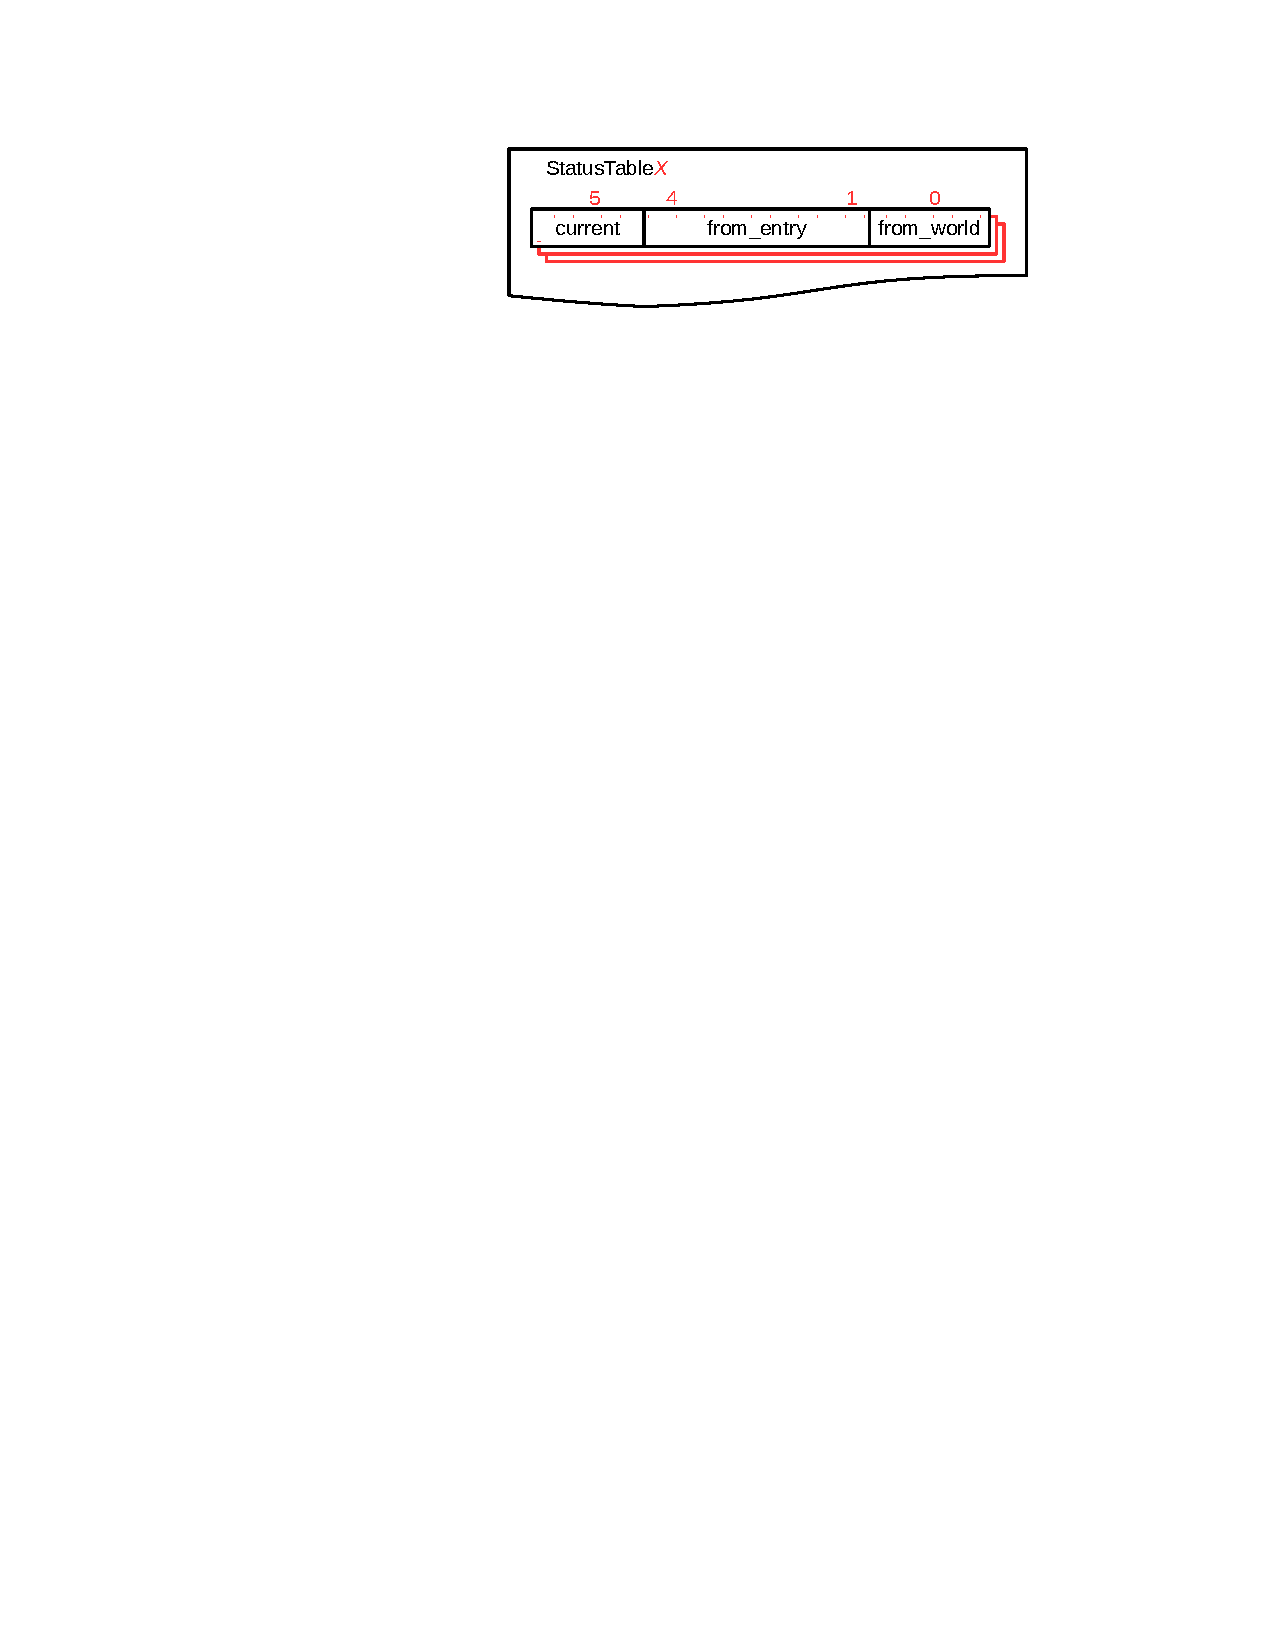
\includegraphics[width=0.5\textwidth]{./38-WCTRL/figures/statustable.pdf}
    \caption{世界切换记录表}
    \label{fig:wcl-world-status}
\end{figure}

具体描述如下：
\begin{itemize}
    \item \hyperref[fielddesc:WCLCORE0FROMWORLDn]{WCL\_CORE\_\regindex{m}\_FROM\_WORLD\_\regindex{n}}：记录世界切换之前的世界信息。
    \begin{itemize}
        \item 0：安全世界
        \item 1：非安全世界
    \end{itemize}
    \item \hyperref[fielddesc:WCLCORE0FROMENTRYn]{WCL\_CORE\_\regindex{m}\_FROM\_ENTRY\_\regindex{n}}：记录发生跳转的入口。
    \begin{itemize}
        \item 0：表示切换之前不处于任何入口监测的中断。
        \item 1 - 13：表示上一个发生中断的入口。
    \end{itemize}
    \item \hyperref[fielddesc:WCLCORE0CURRENTn]{WCL\_CORE\_\regindex{m}\_CURRENT\_\regindex{n}}：表示该入口当前是否处于监测的中断中。当某个入口 \regindex{x} 发生中断时，
    \begin{itemize}
        \item 该入口对应的 \hyperref[fielddesc:WCLCORE0CURRENTn]{WCL\_CORE\_\regindex{m}\_CURRENT\_\regindex{x}} 域均将被更新为 1，
        \item 其余入口的 current 域均将更新为 0。
    \end{itemize}
\end{itemize}

\subsection{世界切换记录表寄存器的更新}\label{sec:wctrl-update-statetable}

假设初始状态下，CPU 处于非安全世界，所有 \hyperref[regdesc:WCLCORE0STATUSTABLEnREG]{WCL\_CORE\_\regindex{m}\_STATUSTABLE\regindex{n}\_REG(\regindex{n}: 1-13)} 寄存器为 0。接着，入口 9、入口 1 和入口 4 依次发生优先级更高的中断。

此时，世界切换记录表更新过程如下：
\begin{enumerate}
    \item 首先，9 号入口监测到中断发生。CPU 开始执行 9 号中断的入口地址时，世界切换记录表更新如图 \ref{fig:wcl-world-change0} 所示：
    \begin{figure}[H]
    \centering
    
\includegraphics[width=0.3\textwidth]{./38-WCTRL/figures/world_table0.eps}
    \caption{中断嵌套流程示意图 - 9 号入口}
    \label{fig:wcl-world-change0}
    \end{figure}
    其中，\begin{itemize}
        \item \hyperref[regdesc:WCLCORE0STATUSTABLEnREG]{WCL\_CORE\_\regindex{m}\_STATUSTABLE9\_REG}
        \begin{itemize}
            \item \hyperref[fielddesc:WCLCORE0FROMWORLDn]{WCL\_CORE\_\regindex{m}\_FROM\_WORLD\_9} 域为 1，表示 CPU 在切换之前处于非安全世界。
            \item \hyperref[fielddesc:WCLCORE0FROMENTRYn]{WCL\_CORE\_\regindex{m}\_FROM\_ENTRY\_9} 域为 0，表示切换之前不处于任何入口监测的中断。
            \item \hyperref[fielddesc:WCLCORE0CURRENTn]{WCL\_CORE\_\regindex{m}\_CURRENT\_9} 域为 1，表示此时 CPU 正在 9 号入口监测的中断中。
        \end{itemize}
        \item 其他 \hyperref[regdesc:WCLCORE0STATUSTABLEnREG]{WCL\_CORE\_\regindex{m}\_STATUSTABLE\regindex{n}\_REG} 寄存器均保持不变。
    \end{itemize}
    \item 接着，1 号入口监测到一个更高优先级的中断。CPU 开始执行 1 号中断的入口地址时，世界切换记录表再次发生更新，如图 \ref{fig:wcl-world-change1} 所示：
        \begin{figure}[H]
        \centering
        
\includegraphics[width=0.3\textwidth]{./38-WCTRL/figures/world_table1.eps}
        \caption{中断嵌套流程示意图 - 1 号入口 }
        \label{fig:wcl-world-change1}
        \end{figure}
    其中，
    \begin{itemize}
        \item \hyperref[regdesc:WCLCORE0STATUSTABLEnREG]{WCL\_CORE\_\regindex{m}\_STATUSTABLE1\_REG}
        \begin{itemize}
            \item \hyperref[fielddesc:WCLCORE0FROMWORLDn]{WCL\_CORE\_\regindex{m}\_FROM\_WORLD\_1} 域为 0，表示 CPU 在切换之前处于安全世界。
            \item \hyperref[fielddesc:WCLCORE0FROMENTRYn]{WCL\_CORE\_\regindex{m}\_FROM\_ENTRY\_1} 域为 9，表示切换之前处于 9 号入口监测的中断。
            \item \hyperref[fielddesc:WCLCORE0CURRENTn]{WCL\_CORE\_\regindex{m}\_CURRENT\_1} 域更新为 1，表示此时 CPU 正在 1 号入口监测的中断中。
        \end{itemize}
        \item \hyperref[regdesc:WCLCORE0STATUSTABLEnREG]{WCL\_CORE\_\regindex{m}\_STATUSTABLE9\_REG}
        \begin{itemize}
            \item \hyperref[fielddesc:WCLCORE0CURRENTn]{WCL\_CORE\_\regindex{m}\_CURRENT\_9} 域更新为 0，表示此时 CPU 已经不在 9 号入口监测的中断中（进入 1 号入口中断的监控中）。
            \item \hyperref[fielddesc:WCLCORE0FROMWORLDn]{WCL\_CORE\_\regindex{m}\_FROM\_WORLD\_9} 域和 \hyperref[fielddesc:WCLCORE0FROMENTRYn]{WCL\_CORE\_\regindex{m}\_FROM\_ENTRY\_9} 域保持不变。
        \end{itemize}
        \item 其他 \hyperref[regdesc:WCLCORE0STATUSTABLEnREG]{WCL\_CORE\_\regindex{m}\_STATUSTABLE\regindex{n}\_REG} 寄存器均保持不变。
    \end{itemize}
        \item 接着，4 号入口又监测到一个更高优先级的中断。CPU 开始执行 4 号中断的入口地址时，世界切换记录表再次发生更新，如图 \ref{fig:wcl-world-change2} 所示：
        \begin{figure}[H]
            \centering
            
\includegraphics[width=0.3\textwidth]{./38-WCTRL/figures/world_table2.eps}
            \caption{中断嵌套流程示意图 - 4 号入口}
            \label{fig:wcl-world-change2}
        \end{figure}
        其中，
        \begin{itemize}
        \item \hyperref[regdesc:WCLCORE0STATUSTABLEnREG]{WCL\_CORE\_\regindex{m}\_STATUSTABLE4\_REG}
        \begin{itemize}
            \item \hyperref[fielddesc:WCLCORE0FROMWORLDn]{WCL\_CORE\_\regindex{m}\_FROM\_WORLD\_4} 域为 0，表示 CPU 在切换之前处于安全世界。
            \item \hyperref[fielddesc:WCLCORE0FROMENTRYn]{WCL\_CORE\_\regindex{m}\_FROM\_ENTRY\_4} 域为 1，表示切换之前处于 1 号入口监测的中断。
            \item \hyperref[fielddesc:WCLCORE0CURRENTn]{WCL\_CORE\_\regindex{m}\_CURRENT\_4} 域更新为 1，表示此时 CPU 正在 4 号入口监测的中断中。
        \end{itemize}
        \item \hyperref[regdesc:WCLCORE0STATUSTABLEnREG]{WCL\_CORE\_\regindex{m}\_STATUSTABLE1\_REG}
        \begin{itemize}
            \item \hyperref[fielddesc:WCLCORE0CURRENTn]{WCL\_CORE\_\regindex{m}\_CURRENT\_1} 域更新为 0，表示此时 CPU 已经不在 1 号入口监测的中断中（进入 4 号入口中断的监控中）。
            \item \hyperref[fielddesc:WCLCORE0FROMWORLDn]{WCL\_CORE\_\regindex{m}\_FROM\_WORLD\_1} 域和 \hyperref[fielddesc:WCLCORE0FROMENTRYn]{WCL\_CORE\_\regindex{m}\_FROM\_ENTRY\_1} 域保持不变。
        \end{itemize}
        \item 其他 \hyperref[regdesc:WCLCORE0STATUSTABLEnREG]{WCL\_CORE\_\regindex{m}\_STATUSTABLE\regindex{n}\_REG} 寄存器均保持不变。
\end{itemize}
\end{enumerate}

\subsection{世界切换记录表寄存器的读取} \label{sec:wctrl-read-table}

通过查看世界切换记录表，我们也可以了解世界切换前的世界以及是否发生中断嵌套等信息，从而能够正确恢复到世界切换前的状态。

具体方式如下（以图 \ref{fig:wcl-world-change2} 为例）：
\begin{enumerate}
    \item 查询 \hyperref[regdesc:WCLCORE0STATUSTABLECURRENTREG]{WCL\_CORE\_\regindex{m}\_STATUSTABLE\_CURRENT\_REG} 寄存器，得知目前 CPU 正处于 4 号入口监测的中断中。
    \item 查询 \hyperref[fielddesc:WCLCORE0FROMENTRYn]{WCL\_CORE\_\regindex{m}\_FROM\_ENTRY\_4} 域为 1，得知之前存在 1 号入口监测的中断。
    \item 查询 \hyperref[fielddesc:WCLCORE0FROMENTRYn]{WCL\_CORE\_\regindex{m}\_FROM\_ENTRY\_1} 域为 9，得知之前存在 9 号入口监测的中断。
    \item 查询 \hyperref[fielddesc:WCLCORE0FROMENTRYn]{WCL\_CORE\_\regindex{m}\_FROM\_ENTRY\_9} 域为 0，得知之前已经不存在其他入口监测的中断；此时，接着查询 \hyperref[fielddesc:WCLCORE0FROMWORLDn]{WCL\_CORE\_\regindex{m}\_FROM\_WORLD\_9} 域为 1，得知世界切换前处于非安全世界。
\end{enumerate}


\subsection{中断嵌套}

\chipname{} 支持中断嵌套，举例而言：

\begin{enumerate}

    \item 假设首先发生中断 A，CPU 跳转至中断 A 的入口地址并触发世界切换。
    \item 接着，在 CPU 正在处理 A 中断时，又发生优先级更高的中断 B。
    \item 此后，CPU 将停止处理中断 A，转而处理优先级更高的中断 B。
    \item 处理完中断 B 后，CPU 将返回中断 A 的入口地址，这会再次触发世界切换。
\end{enumerate}

这种情况会导致 \nameref{subsub:world_switch_table} 记录出错，无法恢复正确的世界。

\subsubsection{处理方法}
为避免中断返回误触发的世界切换，用户需进行如下操作：
\begin{itemize}
    \item 在设计阶段，在所有中断和异常的 vector 入口处插入两条 NOP.N (No Operation) 汇编指令。
    \item 在执行阶段, 对当前中断的返回地址进行特别处理。
\end{itemize}

上述操作可以保证 \regindex{A} 号入口监测的中断在返回时不会返回到 \regindex{B} 号入口的入口地址，而是 NOP 指令之后的地址，从而确保世界切换记录表不会触发。此外，由于所有中断前两条指令均为 NOP 指令，因此即使未返回至起始地址也不会影响程序的正常执行。

\subsubsection{编程指南}

\textbf{处理 \regindex{A} 处的中断：\label{step:wctrl-start-interrput}}
    \begin{enumerate}
        \item 执行清除 write\_buffer 的操作, 向 \hyperref[regdesc:WCLCORE0MESSAGEADDRREG]{WCL\_CORE\_\regindex{m}\_MESSAGE\_ADDR\_REG} 配置的地址中连续写入 0、1、\dots 、\regindex{Z-1}、\regindex{Z} 序列。
        \item 正常执行中断服务程序。\label{step:interrupt-process-normal}
        \item 禁止所有中断使能。
        \item 处理 \regindex{A} 处中断的返回地址： \label{step:interrupt_process_update}
        \begin{itemize}
            \item 查询 \regindex{A} 号入口的世界切换记录寄存器中的 \hyperref[fielddesc:WCLCORE0FROMENTRYn]{WCL\_CORE\_\regindex{m}\_FROM\_ENTRY\_\regindex{A}}：
            \begin{itemize}
                \item 0：表示所有中断均已全部处理，需返回普通应用程序:
                \begin{enumerate}
                    \item 更新 \regindex{A} 的世界切换寄存器： \hyperref[fielddesc:WCLCORE0CURRENTn]{WCL\_CORE\_\regindex{m}\_CURRENT\_\regindex{A}} 为 0，表示中断已不再 \regindex{A} 处。
                    \item 跳转至第 \ref{step:last-step} 步。
                \end{enumerate}

                \item 1 - 13：表示需返回其他 \regindex{B} 号入口监测的中断，
                \begin{enumerate}
                    \item 首先检查并处理当前 \regindex{A} 号入口的中断返回地址，如果：
                    \begin{itemize}
                        \item 指向 \regindex{B} 号入口中断的第一条 NOP.N 指令，则将 \regindex{A} 号中断的返回地址加 4
                        \item 指向 \regindex{B} 号入口中断的第二条 NOP.N 指令，则将 \regindex{A} 号中断的返回地址加 2
                        \item 指向其他地址，返回地址不变
                    \end{itemize}
                    \item 手动更新世界切换记录表：
                    \begin{itemize}
                        \item 更新 \regindex{A} 的世界切换寄存器： \begin{itemize}
                            \item \hyperref[fielddesc:WCLCORE0CURRENTn]{WCL\_CORE\_\regindex{m}\_CURRENT\_\regindex{A}} 为 0，表示中断已不在 \regindex{A} 处。
                            \item \hyperref[fielddesc:WCLCORE0FROMWORLDn]{WCL\_CORE\_\regindex{m}\_FROM\_WORLD\_\regindex{A}} 和 \hyperref[fielddesc:WCLCORE0FROMENTRYn]{WCL\_CORE\_\regindex{m}\_FROM\_ENTRY\_\regindex{A}} 的更新不作要求。
                        \end{itemize}
                        \item 更新 \regindex{B} 的世界切换寄存器：
                        \begin{itemize}
                            \item  \hyperref[fielddesc:WCLCORE0CURRENTn]{WCL\_CORE\_\regindex{m}\_CURRENT\_\regindex{B}} 为 1，表示将返回至 \regindex{B} 入口。
                        \end{itemize}
                     \end{itemize}
            \end{enumerate}
            \end{itemize}
        \end{itemize}
        \item 准备退出中断。\label{step:last-step}
            \begin{enumerate}
                \item 查询需前往的世界：
                    \begin{itemize}
                        \item 如仍处于相同世界，则跳转到第 \ref{step:final} 步。
                        \item 如需前往其他世界，则切换至需要的世界，参考\ref{sec:38-WCTRL-recommended-operation}。然后跳转到第 \ref{step:final} 步。
                    \end{itemize}
            \end{enumerate}
        \item 恢复中断使能, 退出中断。 \label{step:final}
\end{enumerate}


\begin{tiplisting}
上述处理过程中的 \ref{step:interrupt_process_update} 和 \ref{step:last-step} 不能被高级中断打断，因此在执行这两个步骤之前应该将所有的中断关闭，处理完之后再将所有的中断打开。
\end{tiplisting}

\section{NMI 中断屏蔽}

\chipname{} 的某些软件过程（比如 World 控制器的配置过程等）可能希望不被任何中断打断，包括 NMI 中断。

通常来说，我们可以通过 CPU 特殊寄存器，使用软件过程来屏蔽中断，但不包括 NMI 中断。NMI 中断必须通过修改中断源来配置，相对麻烦。（详见 \ref{mod:intmtrx} \textit{\nameref{mod:intmtrx}} ）

为了快速使能或屏蔽 NMI 中断，World 控制器设计了一种硬件机制：
\begin{itemize}
    \item \textbf{所有}应用程序完全屏蔽 NMI 中断：
    \begin{itemize}
        \item 配置 \hyperref[fielddesc:WCLCORE0NMIMASK]{WCL\_CORE\_\regindex{m}\_NMI\_MASK}
            \begin{itemize}
            \item 1：可直接完全屏蔽所有 NMI 中断
            \item 0：可取消屏蔽
            \end{itemize}
    \end{itemize}
    \item \textbf{部分}应用程序屏蔽 NMI 中断：
        \begin{enumerate}
            \item 配置 \hyperref[fielddesc:WCLCORE0NMIMASKTRIGGERADDR]{WCL\_CORE\_\regindex{m}\_NMI\_MASK\_TRIGGER\_ADDR} 为需要结束 NMI 中断的应用程序地址，即 CPU 执行到这个地址开始不再屏蔽 NMI 中断。
            \item 配置 \hyperref[fielddesc:WCLCORE0NMIMASKDISABLE]{WCL\_CORE\_\regindex{m}\_NMI\_MASK\_DISABLE} 为任意值，表明 TRIGGER\_ADDR 配置完成
            \item 配置 \hyperref[fielddesc:WCLCORE0NMIMASKENABLE]{WCL\_CORE\_\regindex{m}\_NMI\_MASK\_ENABLE} 为任意值，开始屏蔽 NMI 中断，直到触发 \\ \hyperref[fielddesc:WCLCORE0NMIMASKTRIGGERADDR]{WCL\_CORE\_\regindex{m}\_NMI\_MASK\_TRIGGER\_ADDR} 后不再屏蔽 NMI 中断。
        \end{enumerate}
\end{itemize}

\begin{tiplisting}
\vspace{-2em}
 \begin{itemize}
    \item 上述两种屏蔽方式不建议混用，需选择其中一种进行使用。
    \item NMI 中断屏蔽配置后长期有效，直至触发。触发之后需要重新配置。
 \end{itemize}
\end{tiplisting}




\clearpage
\section{寄存器列表}\hypertarget{wctrl-reg-summ}{}

本小节的所有地址均为相对于 World 控制器基地址的地址偏移量（相对地址），具体基地址请见章节 \ref{mod:sysmem} \textit{\nameref{mod:sysmem}} 中的表 \ref{tab:sysmem-base-address}。

注意，CPU0 与 CPU1 的寄存器完全相同。
下方表格仅列出 CPU0 的相关寄存器，CPU1 的寄存器仅需在 CPU0 相关寄存器地址偏移量的基础上再加 0x{}0400 即可。

比如 \hyperref[regdesc:WCLCORE0ENTRYCHECKREG]{WCL\_CORE\_0\_ENTRY\_CHECK\_REG} 的地址偏移量为 0x{}007C，则 \hyperref[regdesc:WCLCORE0ENTRYCHECKREG]{WCL\_CORE\_1\_ENTRY\_CHECK\_REG} 的地址偏移量为 0x{}047C。

请查看章节 \hyperref[glossary-access-types]{\textit{寄存器的访问类型}}，了解“访问”列缩写的含义。

\subfile{\modulefiles/38-WCTRL-reg-summ__CN}


\clearpage
\section{寄存器}

本小节的所有地址均为相对于 World 控制器基地址的地址偏移量（相对地址），具体基地址请见章节 \ref{mod:sysmem} \textit{\nameref{mod:sysmem}} 中的表 \ref{tab:sysmem-base-address}。

注意，CPU0 与 CPU1 的寄存器完全相同。
下方仅列出 CPU0 的相关寄存器，CPU1 的寄存器仅需在 CPU0 相关寄存器地址偏移量的基础上再加 0x{}0400 即可。

比如 \hyperref[regdesc:WCLCORE0ENTRYCHECKREG]{WCL\_CORE\_0\_ENTRY\_CHECK\_REG} 的地址偏移量为 0x{}007C，则 \hyperref[regdesc:WCLCORE0ENTRYCHECKREG]{WCL\_CORE\_1\_ENTRY\_CHECK\_REG} 的地址偏移量为 0x{}007C + 0x{}0400，即 0x{}047C。

\subfile{\modulefiles/38-WCTRL-reg__CN}

\end{document}
